\medskip

% \graphicspath{{Figures/}}

\section*{CRediT author statement}
\textbf{Ibrahim Hmamou:} Software, Writing ‐ Original Draft, Writing ‐ Review \& Editing \\
\textbf{Olivier Delestre:} Resources, Supervision\\
\textbf{Carine Lucas:} Writing ‐ Original Draft, Supervision, Project administration

\section*{Reproducibility Summary}

\paragraph{Scope of Reproducibility --}In~\cite{Andrea}, the authors proposed a set of equations to model the flow of particulate suspensions driven by sedimentation. In particular, they aimed at modelling laboratory experiments which consist in the dam-break flow of a particulate suspension, of variable solid concentration, that progressively settles during propagation. They implemented the discretization of these equations and they compared their numerical results to the set of experiments.
Our goal is, starting from the same model, to discretize the equations as explained in the article, in order to check if all the necessary information on the numerical method they used is available in the article.

\paragraph{Methodology --}Starting from scratch, the objective of the first author was to become familiar with the numerical schemes used to simulate flows thanks to approximations of conservation laws.
He began with the classical one-dimensional one-layer Shallow-Water equations and improved his software up to the resolution of the three layer model of~\cite{Andrea}, with well suited numerical tricks.

\paragraph{Results --}The numerical results obtained in this replication are qualitatively the same as the one of the original article. The experimental data and the numerical approximation of the model fit well.

%\paragraph{What was easy --}\textcolor{red}{si on veut, à voir}

%\paragraph{What was difficult --}\textcolor{red}{si on veut, à voir - On peut aussi mettre d'autres choses si besoin. }

\paragraph{Communication with original authors --}We communicated with the authors to get the experimental data as they were not available at this moment. \\
After this work, we also obtained their numerical results in order to perform a precise (quantitative) comparison of the results. This comparison is detailed in Section~\ref{sec:comp} and shows little differences.

\section{Introduction}

In the original work~\cite{Andrea}, a new mathematical model was introduced to simulate geophysical flows such as lahars. They contain suspended particles that move and settle under the effect of gravity. A series of laboratory experiments were performed in the experimental device schematized in figure~\ref{fig:expe}, with glass beads to model natural materials (see~\cite{expe} and the corresponding data at \url{https://doi.org/10.57745/IV4SE8}). The column of sediments in the reservoir is first fully fluidized in order to obtain a homogeneous suspension. Then, the door is opened and the suspension flows into the channel, until it reaches a steady state, with deposit on the bottom covered with clean water.   \\
%\textcolor{blue}{Par rapport à ce qui est dit plus bas (sur la longueur 3.5m), faudra peut-être changer l'image ?} \textcolor{red}{fait}

\begin{center}
\begin{figure}[ht!]
    \centering
    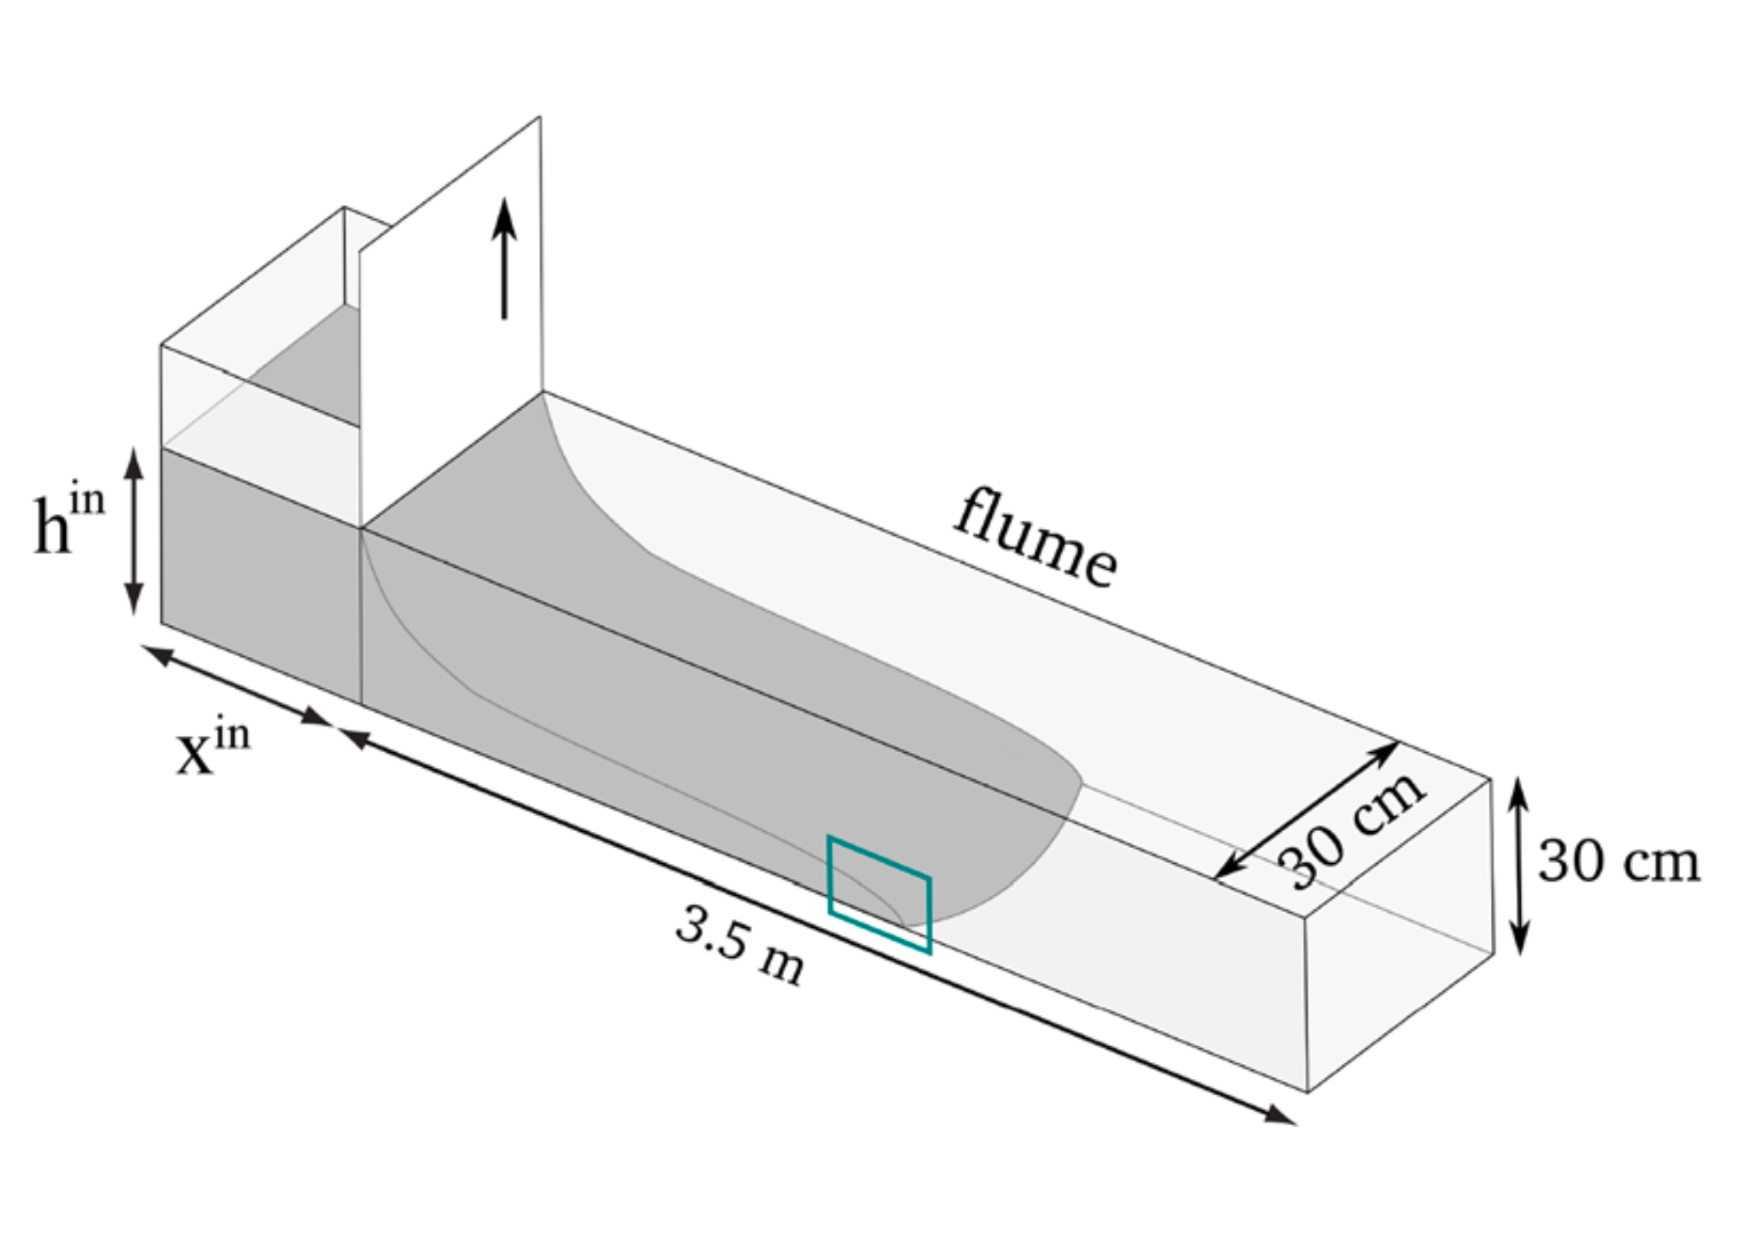
\includegraphics[width = 0.8\textwidth]{Figures/Flume.pdf}
    \caption{Experimental device, from~\cite{Andrea}.}
    \label{fig:expe}
\end{figure}
\end{center}

In \cite{Andrea}, numerical results are then compared with experiments.
The equations that describe the mathematical model are available in the original work, but the code solving their numerical approximations was not made available.\\

This article is structured as follow: first, we recall the model of the original article~\cite{Andrea}. Then, thank to the references, we re-write the complete numerical scheme and we precise the choices we made when necessary.
In a following section, we plot the numerical results given by the C++ software we wrote (SednaSh, available at \url{https://plmlab.math.cnrs.fr/ltoti92/sednash}).
Finaly, the last section is devoted to a more precise comparison with the numerical results obtained by the authors of the original article.

\section{Model}
Let us recall the original model~\cite[eq.~(10)--(14)]{Andrea}:
\begin{subequations}
\label{eq:model}
\newlength{\mylhs}
\settowidth{\mylhs}{$\partial_t(H\bar{U}) + \partial_x(H\bar{U}^2)$}
\begin{align}
\hspace{-4cm}\text{\rotatebox[origin=c]{90}{fluid}} & \left\{
\begin{aligned}
    \mathmakebox[\mylhs][l]{\partial_t H + \partial_x(H\bar{U})} &= \left( \dfrac{\phi_{pack}}{\phi_s} - 1 \right) S_{sed}, \\
    \mathmakebox[\mylhs][l]{\partial_t(H\bar{U}) + \partial_x(H\bar{U}^2)} &= \left( \dfrac{\phi_{pack}}{\phi_s} - 1 \right) S_{sed} \, \bar{U} - g H \, \partial_x(H + h + h_d),
\end{aligned} \right. \label{eq:fluid} \\
\text{\rotatebox[origin=c]{90}{suspension}} & \left\{
\begin{aligned}
    \mathmakebox[\mylhs][l]{\partial_t h + \partial_x(h\bar{u})} &= S_{slump} - \dfrac{\phi_{pack}}{\phi_s} S_{sed}, \\
    \mathmakebox[\mylhs][l]{\partial_t(h\bar{u}) + \partial_x(h\bar{u}^2)} &= \left( S_{slump} - \dfrac{\phi_{pack}}{\phi_s} S_{sed} \right) \bar{u} \\
    & \quad - \kappa \bar{u} \, \chi(t > t_{f\!f}) - g h \, \partial_x \left( \dfrac{\rho_f}{\rho_m} H + h + h_d \right),
\end{aligned} \right. \label{eq:suspension} \\
\text{\rotatebox[origin=c]{90}{deposit}} & \left\{
\begin{aligned}
    \mathmakebox[\mylhs][l]{\partial_t h_d} \hspace{4.5pt} &= S_{sed}.
\end{aligned} \right. \label{eq:deposit}
\end{align}
\end{subequations}
~\\[-0.7\baselineskip]

This is a three layers model. More precisely, from top to bottom, there are three physical layers, namely 1) a fluid layer, without particles, of height $H$ and velocity $\bar{U}$, 2) a suspension layer characterized by its height $h$ and its velocity $\bar{u}$, and 3) a deposit layer of height $h_d$ where particles do not move.
Each layer is has a small aspect ratio: the velocities are assumed not to depend on the vertical position in the layer ($\bar{u}$ and $\bar{U}$ are mean velocities). The model is a Shallow Water type model.

The system~\eqref{eq:model} contains several parameters that are detailed in the original article. Let us recall that $\phi_{pack}$ is the volume fraction of the deposit, $\phi_s$ is the volume fraction of the suspension; $\kappa$ is the basal friction coefficient.
Finally, as the shallow water approximation is not valid in the reservoir, the authors used the approach of~\cite{Larrieu} and they considered a gravitational collapse, during  a characteristic time $t_{f\!f} = \sqrt{2 (h^{in} - h_{app})/g}$
that corresponds to the time needed for a particle to fall from the initial height $h^{in}$ to the apparent height $h_{app} = \varepsilon x^{in} \ll x^{in}$, with $x^{in}$ the length of the reservoir.
Finally, $S_{sed}$ and $S_{slump}$ are source terms detailed hereafter, $g$ is the gravity constant, $\rho_f$ is the density of the fluid and $\rho_m$ is the density of the suspension layer.

The source term $S_{slump}$ converts the movement of the suspension into a continuous flow and reads
$S_{slump}(t,x) = gt \chi( 0 \leq x \leq x^{in})\chi( 0 \leq t \leq t_{f\!f})$. The source term $S_{sed}$ representing the suspended particles that sediment and constitute the deposit layer is written as
$S_{sed}(t) = R_{sed} \, \chi(t > t_{f\!f}) $ with $$R_{sed} = \dfrac{\rho_s}{\rho_s - \rho_f} \dfrac{U_{sed}^{calculated}}{\dfrac{\phi_{pack}}{\phi_s} - 1}. $$

In these equalities, $\chi(I)$ is the indicator function of the subset~$I$.
The numerical value of the dynamic settling velocity of the grains reads $U_{sed}^{calculated} = U_{sed}^{static}/C_{sed}$.
The $C_{sed}$ coefficient is a correction of the sedimentation velocity ($C_{sed} = 1 / C(Re)$ with the notation of \cite{Andrea}) calibrated from the location of the front at the end of the experiments using the optimization algorithm~\ref{algo:calib_final}. Note that we decided here to use the notation $U^{calculated}_{sed}$ instead of $U_{sed}^{dynamic}$ as in \cite{Andrea} because its value is not physical but numerically fitted to recover the correct runout distances of the flows (see \cite[caption of figure 10 (b)]{Andrea}).

\begin{algorithm}[H]
    \caption{Optimization of the $C_{sed}$ parameter}
    \label{algo:calib_final}

    \SetKwInOut{Input}{Input}
    \SetKwInOut{Output}{Output}

    \Input{Experimental target $x_{exp}^{max}$, Search range $\Omega$}
    \Output{Optimized parameter $C_{sed}$}

    \BlankLine
    \textbf{Function} \text{EvaluateError}($C$):\\
    \Indp
        Run simulation with parameter $C$ to obtain $x_{sim}^{max}$\;
        Compute $\epsilon \leftarrow |x_{sim}^{max} - x_{exp}^{max}|$\;
        \Return $\epsilon$\;
    \Indm

    \BlankLine
    Find $C_{sed}$ that minimizes \text{EvaluateError} over $\Omega$\;

    \Return $C_{sed}$\;
\end{algorithm}


Introducing the following new variables (as written in the SednaSh code):
\begin{align*}
    Sed_{up} &= \frac{\rho_s}{\rho_s - \rho_f} U_{sed}^{num} & &\mbox{\hspace{-0.8cm} such that } \left( \frac{\phi_{pack}}{\phi_s} - 1 \right) S_{sed}= Sed_{up} \, \chi(t > t_{f\!f}), \\
    Sed_{low} &= \frac{\phi_{pack}}{\phi_{pack} - \phi_{s}} \frac{\rho_s}{\rho_s - \rho_f} U_{sed}^{num} & &\mbox{\hspace{-0.8cm} such that } \qquad \ \  \quad\frac{\phi_{pack}}{\phi_s} S_{sed}= Sed_{low} \, \chi(t > t_{f\!f}), \\
    Agg &= \frac{\phi_{s}}{\phi_{pack} - \phi_{s}} \frac{\rho_s}{\rho_s - \rho_f} U_{sed}^{num} = R_{sed},& &
\end{align*}
and setting $\kappa = C_{fric} \, R_{sed} \,  \phi_{pack}/\phi_s = C_{fric} \, Sed_{low}$,
we can rewrite system~\eqref{eq:model} as follows:
\begin{subequations} \label{eq:model_newvars}
\begin{align*}
\partial_t H + \partial_x(H\bar{U})
&= Sed_{up} \ \chi(t > t_{f\!f}),
\\[1em]
\partial_t(H\bar{U}) + \partial_x(H\bar{U}^2)
&= Sed_{up} \, \chi(t > t_{f\!f}) \, \bar{U}
- g H \, \partial_x(H + h + h_d),
\\[1em]
\partial_t h + \partial_x(h\bar{u})
&= gt\, \chi( 0 \leq x \leq x^{in})\chi( 0 \leq t \leq t_{f\!f}) - Sed_{low} \, \chi(t > t_{f\!f}),
\\[1em]
\partial_t(h\bar{u}) + \partial_x(h\bar{u}^2)
&= gt\, \chi( 0 \leq x \leq x^{in})\chi( 0 \leq t \leq t_{f\!f}) \bar{u} \\
& \qquad- \left(1 + C_{fric}\right)Sed_{low} \, \bar{u} \, \chi(t > t_{f\!f}) - g h \, \partial_x \left( \frac{\rho_f}{\rho_m} H + h + h_d \right),
\\
\partial_t h_d &= Agg \, \chi(t > t_{f\!f}).
\end{align*}
\end{subequations}


\section{Numerical approximation}

As in \cite{Andrea}, we are interested in writing a numerical approximation of system~\eqref{eq:model}, following the ideas of~\cite{BerFouMor} where they introduce new variables:
\begin{equation*}
h_1 = H + h + h_d, \qquad
h_2 = \frac{\rho_f}{\rho_m} H + h + h_d, \qquad
\mathcal{X}_1 = \frac{H}{h_1}, \qquad
\mathcal{X}_2 = \frac{h}{h_2}.
\end{equation*}
Then we obtain:
\begin{subequations}
    \label{eq:sysnewvars}
    \begin{align}
    \partial_t H + \partial_x \left( \mathcal{X}_1 h_1 \bar{U}\right)& = Sed_{up} \, \chi(t > t_{f\!f})\\
    \partial_t \left( H \bar{U}\right) + \partial_x \left( \mathcal{X}_1 \left( h_1 \bar{U}^2 + \frac{g}{2} h_1^2\right) \right) & = Sed_{up} \, \chi(t > t_{f\!f}) \, \bar{U} \nonumber \\
    & \qquad + \frac{g}{2} \partial_x \left( H \left( h_1 - H\right)\right) - g H \partial_x (h_1 - H)\\
    \partial_t h + \partial_x \left( \mathcal{X}_2 h_2 \bar{u}\right) &= gt\, \chi( 0 \leq x \leq x^{in})\chi( 0 \leq t \leq t_{f\!f}) \nonumber \\
    & \qquad- Sed_{low} \, \chi(t > t_{f\!f})\\
    \partial_t \left( h \bar{u}\right) + \partial_x \left( \mathcal{X}_2 \left( h_2 \bar{u}^2 + \frac{g}{2} h_2^2\right) \right) &= gt\, \chi( 0 \leq x \leq x^{in})\chi( 0 \leq t \leq t_{f\!f}) \, \bar{u} \nonumber \\
    & \qquad- (1 + C_{fric})Sed_{low} \, \bar{u} \, \chi(t > t_{f\!f}) \nonumber\\
    &\qquad + \frac{g}{2} \partial_x \left( h \left( h_2 - h \right)\right) - g h \partial_x (h_2 - h)\\
    \partial_t h_d &= Agg \, \chi(t > t_{f\!f}).
\end{align}
\end{subequations}
System~\eqref{eq:sysnewvars} can be rewritten under a vector form as:
\begin{subequations}\label{eq:sysBert}
\begin{align}
 \partial_t w_1 + \partial_x \left( \mathcal{X}_1 f(W_1) \right) &= P(H,h_1) + S_1(\bar{U})\\
 \partial_t w_2 + \partial_x \left( \mathcal{X}_2 f(W_2) \right) &= P(h,h_2) + S_2(\bar{u})\\
 \partial_t h_d &= Agg \ \chi(t > t_{f\!f})
 \end{align}
\end{subequations}
with \\
\vspace{-0.2cm}
\begin{minipage}{0.45\textwidth}
\begin{align*}
    w_1 &= (H,H\bar{U})^T \\
    w_2 &= (h,h\bar{u})^T\\
    f(W_1) &= (h_1 \bar{U}, h_1 \bar{U}^2 + \frac{g}{2} h_1^2)^T\\
\end{align*}
\end{minipage}
\hfill
\begin{minipage}{0.45\textwidth}
\begin{align*}
    W_1 &= (h_1,h_1\bar{U})^T \\
    W_2 &= (h_2, h_2\bar{u})^T\\
    f(W_2) &= (h_2 \bar{u}, h_2 \bar{u}^2 + \frac{g}{2} h_2^2)^T\\
\end{align*}
\end{minipage}\\
\vspace{-0.6cm}
and\\[-0.2cm]
\begin{align*}
    S_1(\bar{U}) & = \begin{pmatrix} Sed_{up} \, \chi(t > t_{f\!f})\\[0.1cm] Sed_{up} \, \chi(t > t_{f\!f})\; \bar{U} \end{pmatrix}\\
    S_2(\bar{u})& = \begin{pmatrix} gt\, \chi( 0 \leq x \leq x^{in})\chi( 0 \leq t \leq t_{f\!f}) - Sed_{low} \, \chi(t > t_{f\!f}) \\[0.1cm]
    gt\, \chi( 0 \leq x \leq x^{in})\chi( 0 \leq t \leq t_{f\!f}) \, \bar{u} - (1 + C_{fric})Sed_{low} \, \bar{u} \, \chi(t > t_{f\!f}) \end{pmatrix}\\
    P(\zeta,\xi) &= \begin{pmatrix} 0\\ \dfrac{g}{2} \partial_x \left(\zeta ( \xi - \zeta)\right)- g \zeta \partial_x (\xi - \zeta)\end{pmatrix}.
\end{align*}
We approximate our system~\eqref{eq:sysBert} using a finite volume scheme: we introduce a time step $\Delta t > 0$ and a space step $\Delta x > 0$, such that we have a uniform mesh, with $(t^n)_{n\in\mathbb{N}}$, and $(x_{i+\frac{1}{2}})_{i\in\mathbb{N}}$ in $\mathbb{R}_+$, such that $t^n = n \Delta t $ and $x_{i + \frac{1}{2}} = (i + \frac{1}{2}) \Delta x$, and we define the cell centered in $x_i$  as $(x_{i - \frac{1}{2}},x_{i + \frac{1}{2}})$. We consider the approximations of the original variables:
$$w^n_{1,i} = (H^n_i,H^n_i\bar{U}^n_i)^T \mbox{ and } w^n_{2,i} = (h^n_i,h^n_i\bar{u}^n_i)^T.$$
Then we can write the scheme as:
\begin{align*}
    w_{1,i}^{n+1} &= w_{1,i}^* + \Delta t \begin{pmatrix}
        Sed_{up} \, \chi(t^n > t_{f\!f})\\
        Sed_{up} \, \chi(t^n > t_{f\!f}) \,  \bar{U}_i^*
    \end{pmatrix}\\
    w_{2,i}^{n+1} &= w_{2,i}^* \\
     & \hspace{-0.2cm}+ \Delta t
    \begin{pmatrix}
        S^n_{res}\, \chi( 0 \leq x_i \leq x^{in})\chi( 0 \leq t^n \leq t_{f\!f}) - Sed_{low} \, \chi(t^n > t_{f\!f})\\
        S^n_{res} \, \chi( 0 \leq x_i \leq x^{in})\chi( 0 \leq t^n \leq t_{f\!f})\, \bar{u}_i^* - (1 + C_{fric})\, Sed_{low} \,  \bar{u}_i^* \, \chi(t^n > t_{f\!f})
    \end{pmatrix}
    \\
    h_{d,i}^{n+1} & = h_{d,i}^n + \Delta t Agg \ \chi(t^n > t_{f\!f}).
\end{align*}
%\textcolor{blue}{Normalement j'ai vérifié et le $x$ c'est un $x_i$, c'est le centre de la cellule}
For $j = 1,2$, the intermediate variables $w_{j,i}^*$ are computed as (see~\cite{BerFouMor}):
\begin{multline*}
    w_{j,i}^* = w_{j,i} - \frac{\Delta t}{\Delta x} (\mathcal{X}^n_{j,i+\frac{1}{2}}f_{\Delta x}(W_{j,i}^n,W_{j,i+1}^n) - \mathcal{X}^n_{j,i-\frac{1}{2}}f_{\Delta x}(W_{j,i-1}^n,W_{j,i}^n)) \\+ \frac{g}{2}\frac{\Delta t}{\Delta x} \begin{pmatrix}
        0 \\
        h_{j,i-\frac{1}{2}}^n h_{j,i+\frac{1}{2}}^n ( \mathcal{X}^n_{j,i+\frac{1}{2}} - \mathcal{X}^n_{j,i-\frac{1}{2}})
    \end{pmatrix}
\end{multline*}
with $f_{\Delta x} = (f^h_{\Delta x},f^{hu}_{\Delta x})$ the approximated classical shallow water numerical flux.
According to the authors of \cite{BerFouMor}, the numerical scheme as formulated is well-balanced, positivity-preserving, consistent, admissible-space-preserving, second-order accurate, computationally efficient, and straightforward to implement.

The HLL (Harten, Lax, van Leer) flux is described in detail in \cite{HLL, Toro} and when applied to a two layers system, considering each layer ($j=1$ or $j=2$) separately, we obtain:
% \begin{align*}
%     f_{\Delta x}(U_i^L,U_i^R) = \begin{cases}
%         F(U_i^L) &\text{if $0 < c_1^{(i)}$}\\
%         \dfrac{c_1^{(i)} F(U_i^L) - c_2^{(i)} F(U_i^R)}{c_2^{(i)} - c_1^{(i)}}+ \dfrac{c_1^{(i)} c_2^{(i)}}{c_2^{(i)}-c_1^{(i)}}(U_i^R-U_i^L) &\text{if $c_1^{(i)} < 0 < c_2^{(i)}$}\\
%         F(U_i^R) &\text{if $c_2^{(i)} < 0$}
%     \end{cases}
% \end{align*}
% with a generic state $U = (h,hu)$, $F(U) = (hu, hu^2 + gh^2/2)$ and with two parameters $c_1^{(i)} < c_2^{(i)} $ defined as
% \begin{subequations}
%     \label{eq:c1c2}
% \begin{align}
%     c_1^{(i)} &= \inf_{U_i = U_i^L, U_i^R} \left( \inf_{j = {1,2}} \lambda_j(U_i)\right)  = \inf_{U_i = U_i^L, U_i^R} \lambda_1(U_i) \\
%     c_2^{(i)} &= \sup_{U_i = U_i^L, U_i^R} \left( \sup_{j = {1,2}} \lambda_j(U_i)\right) = \sup_{U_i = U_i^L, U_i^R} \lambda_2(U_i)
% \end{align}
% \end{subequations}
% where $\lambda_1(U_i) = u_i-\sqrt{gh_i}$ and $\lambda_2(U_i) = u_i+\sqrt{gh_i}$.
\begin{align*}
    f_{\Delta x}(U_j^L,U_j^R) = \begin{cases}
        F(U_j^L) &\text{if $0 < c_1^{(j)}$}\\
        \dfrac{c_1^{(j)} F(U_j^L) - c_2^{(j)} F(U_j^R)}{c_2^{(j)} - c_1^{(j)}}+ \dfrac{c_1^{(j)} c_2^{(j)}}{c_2^{(j)}-c_1^{(j)}}(U_j^R-U_j^L) &\text{if $c_1^{(j)} < 0 < c_2^{(j)}$}\\
        F(U_j^R) &\text{if $c_2^{(j)} < 0$}
    \end{cases}
\end{align*}
with a generic state $U = (h,hu)$, $F(U) = (hu, hu^2 + gh^2/2)$ and with two parameters $c_1^{(j)} < c_2^{(j)} $ defined as
\begin{subequations}
    \label{eq:c1c2repro}
\begin{align}
    c_1^{(j)} &= \inf_{U_j = U_j^L, U_j^R} \left( \inf_{k = {1,2}} \lambda_k(U_j)\right)  = \inf_{U_j = U_j^L, U_j^R} \lambda_1(U_j) \label{eq:c1repro} \\
    c_2^{(j)} &= \sup_{U_j = U_j^L, U_j^R} \left( \sup_{k = {1,2}} \lambda_k(U_j)\right) = \sup_{U_j = U_j^L, U_j^R} \lambda_2(U_j) \label{eq:c2repro}
\end{align}
\end{subequations}
where $\lambda_1(U_j) = u_j-\sqrt{gh_j}$ and $\lambda_2(U_j) = u_j+\sqrt{gh_j}$.
The following CFL condition must be satisfied:
\begin{equation*}
    \frac{\Delta t }{\Delta x} \max_{j=1,2, \, i\in\mathbb{N}} (\vert \lambda_1(W_{j,i}^n,W_{j,i+1}^n)\vert, \vert \lambda_2(W_{j,i}^n,W_{j,i+1}^n)\vert )
    \leq C_{CFL}
\end{equation*}
where, for the simulations, $C_{CFL} = 1/2$ was chosen, and we must also verify
\begin{equation*}
    \frac{\Delta t }{\Delta x}  \left( \max(0,f_{\Delta x}(W_{j,i}^n,W_{j,i+1}^n)) - \min (0,f_{\Delta x}(W_{j,i-1}^n,W_{j,i}^n))
    \right) \leq h_{j,i}^n.
\end{equation*}
To match the physical configuration of the experiment, we impose a wall condition on the left, and, since the deposit does not go all the way through the channel, we chose an open boundary condition. We have checked that this choice does not change anything about the deposit.

Note that to properly handle the wet-dry transition for both the upper and lower layers, a numerical depth threshold of $10^{-12}$ m is introduced. This specific value is chosen to be safely above the double-precision machine epsilon ($\approx 2.2 \times 10^{-16}$), thereby preventing division by zero and round-off errors, while remaining physically negligible compared to any characteristic water depth encountered in the simulations. If the water depth in either the fluid or suspension layer falls below this tolerance, that specific layer is considered locally dry, and its corresponding depth, velocity, and discharge are explicitly set to zero.

\section{Results}
The experiments were performed in a channel of total length $L=3.605$~m, with a reservoir of length $x^{in}=0.105$~m (see figure \ref{fig:expe}) during $T_{end}=4$~s (but the suspension layer disappears before this time). In the reservoir, the suspension expands up to $h^{in}=0.27$~m height, but, after the gravitational collapse lasting $t_{f\!f}\approx 0.23$~s, falls to
$h_{app}=\varepsilon x^{in}$ with $\varepsilon=10^{-1}$.

 The experiments where performed with several values of the dilatation rate:
 $$E=\{1.12, 1.17, 1.22, 1.28, 1.35, 1.42\}.$$
 The volume fraction of the deposit is $\phi_{pack} = 0.58$ and the volume fraction of the suspension is $\phi_{s}=\phi_{pack}/E$. The densities are $\rho_{s} = 2500$~kg~m\textsuperscript{-3} for the suspension, $\rho_{f} = 998$~kg~m\textsuperscript{-3} for the fluid and $\rho_{m}= \phi_s \rho_s + (1 - \phi_s) \rho_f$ is the mixture density. The diameter of the particles is $d=350\times 10^{-6}$~m,
 and their sedimentation velocity is computed as $$U_{sed} = \frac{g(\rho_s - \rho_f) d^2}{18 \mu_f (1-\phi_s) F_1 F_2}$$
 where $\mu_f = 10^{-3}$~kg m\textsuperscript{−1} s\textsuperscript{−1} is the dynamic viscosity, $$F_1 = \dfrac{E}{1.9} + 0.85 E^{-2} (1-E^{-1})^{-2/3} \mbox{ and }
 F_2 = \dfrac{{St_0}+45}{{35 St_0}+45}$$ with the Stokes number $$St_0 = \dfrac{(\rho_s - \rho_f)(\rho_s + \frac{\rho_f}{2} g d^3)}{18 \mu_f^2}.$$ \\
 The friction coefficient is $C_{fric}=0.5$ and the $C_{sed}$ values computed thanks to Algorithm~\ref{algo:calib_final} with $\Omega = ]0.5,5[$ are
 \begin{equation}
     C_{sed}=\{1.193, 1.103, 1.461, 1.648, 2.432, 3.113\}.
     \label{eq:csed}
\end{equation}
%  $$C_{sed}=\{1.193, 1.103, 1.461, 1.648, 2.432, 3.113\}.$$
 The gravity is taken as $g=9.81$~m s\textsuperscript{-2}. \\
 For the numerical simulations, the space step is $dx=0.005$~m. \\





Following the approach of the original paper, several numerical experiments were performed, depending on the value of the expansion ranging from 12\% to 42\%. They are compared to experimental measures in figure~\ref{fig:res}.
\begin{figure}[ht!]
    \centering
    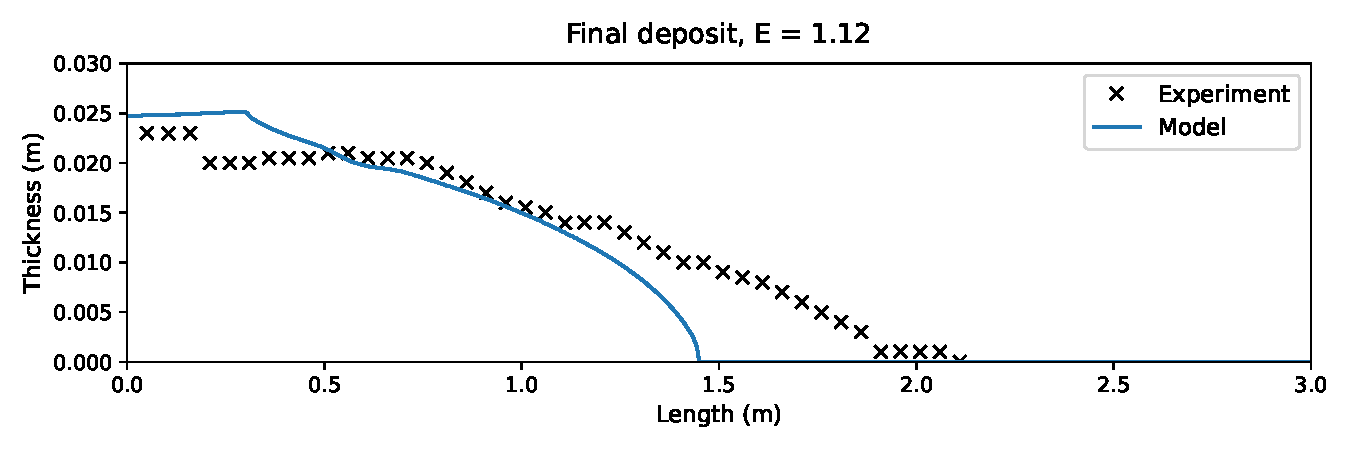
\includegraphics[width=0.45 \textwidth]{Figures/my_csed_E_1.12.pdf}
    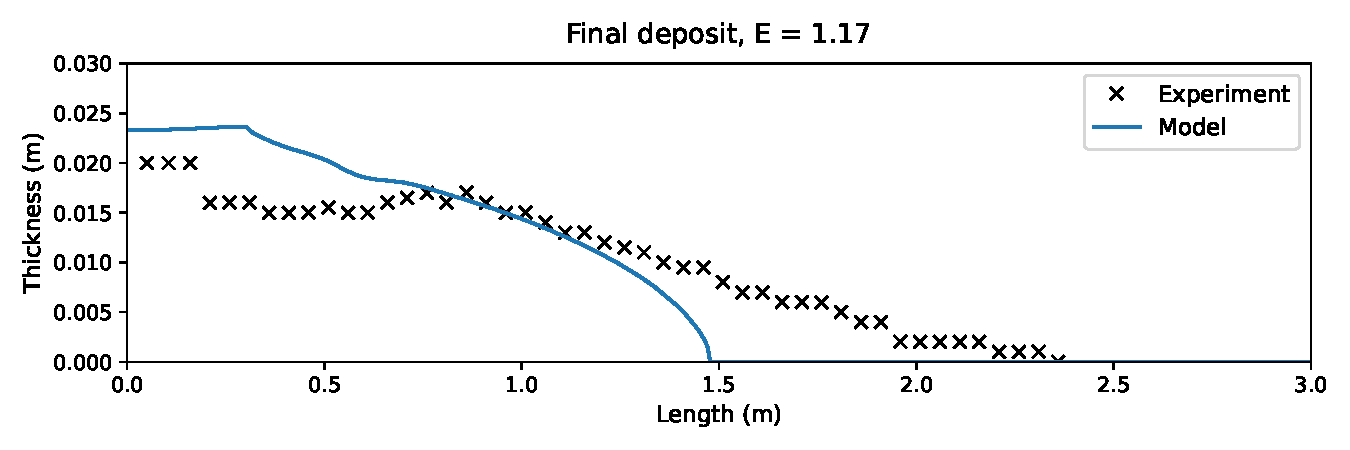
\includegraphics[width=0.45 \textwidth]{Figures/my_csed_E_1.17.pdf}\\
    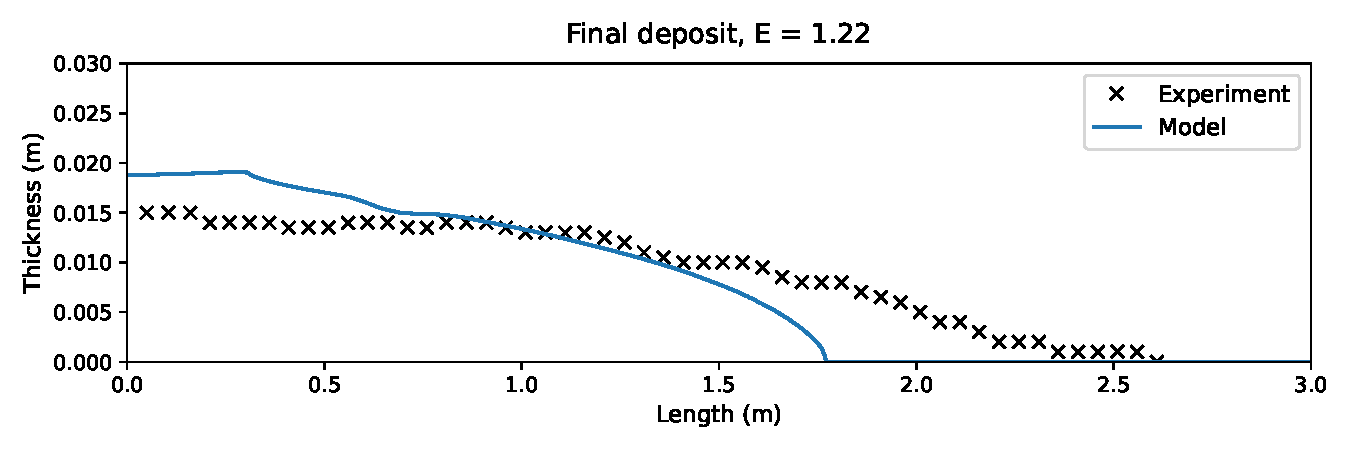
\includegraphics[width=0.45 \textwidth]{Figures/my_csed_E_1.22.pdf}
    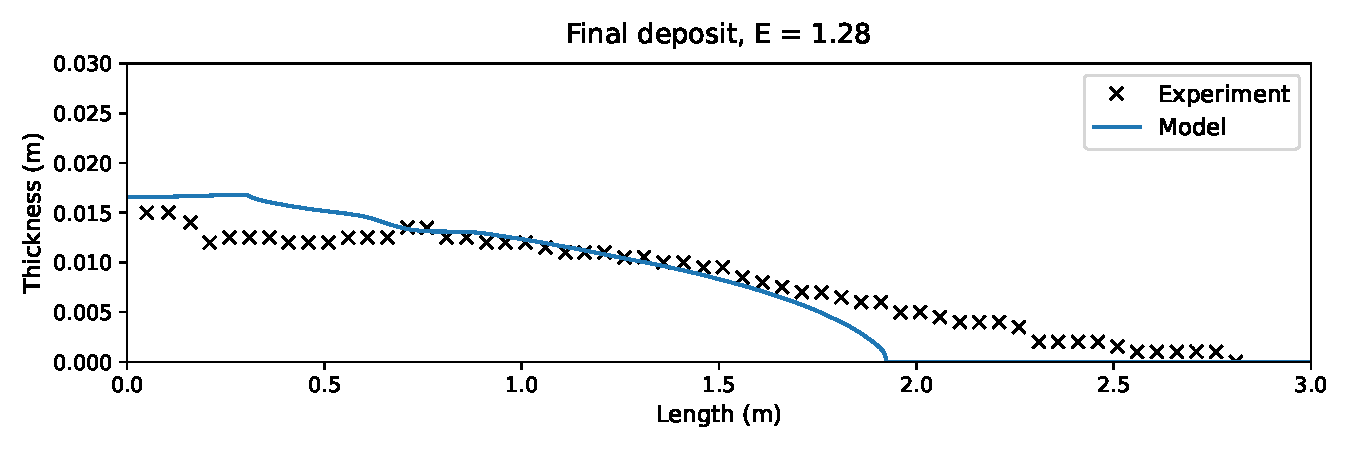
\includegraphics[width=0.45 \textwidth]{Figures/my_csed_E_1.28.pdf}\\
    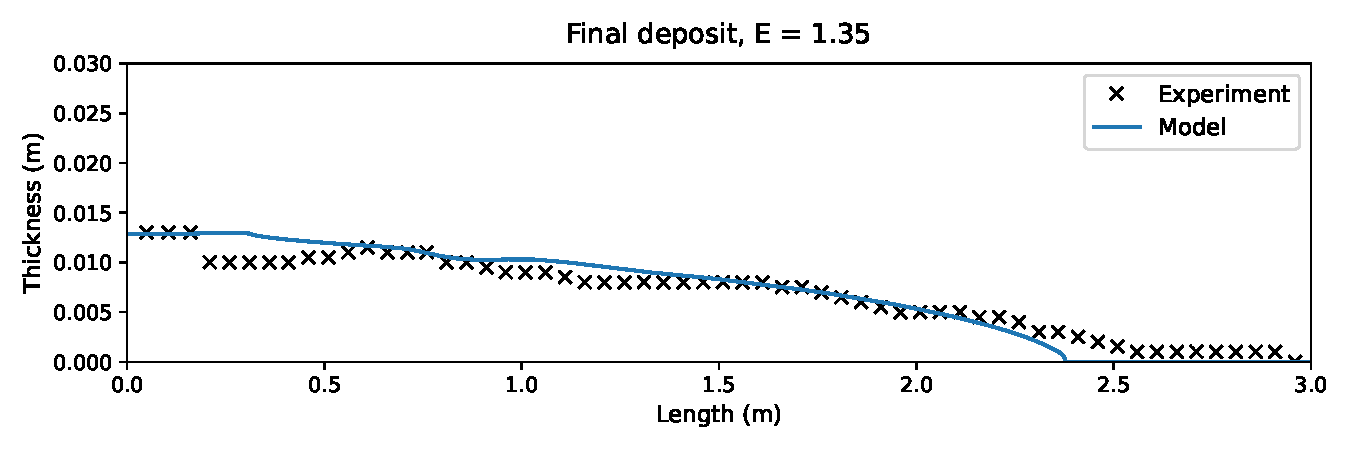
\includegraphics[width=0.45 \textwidth]{Figures/my_csed_E_1.35.pdf}
    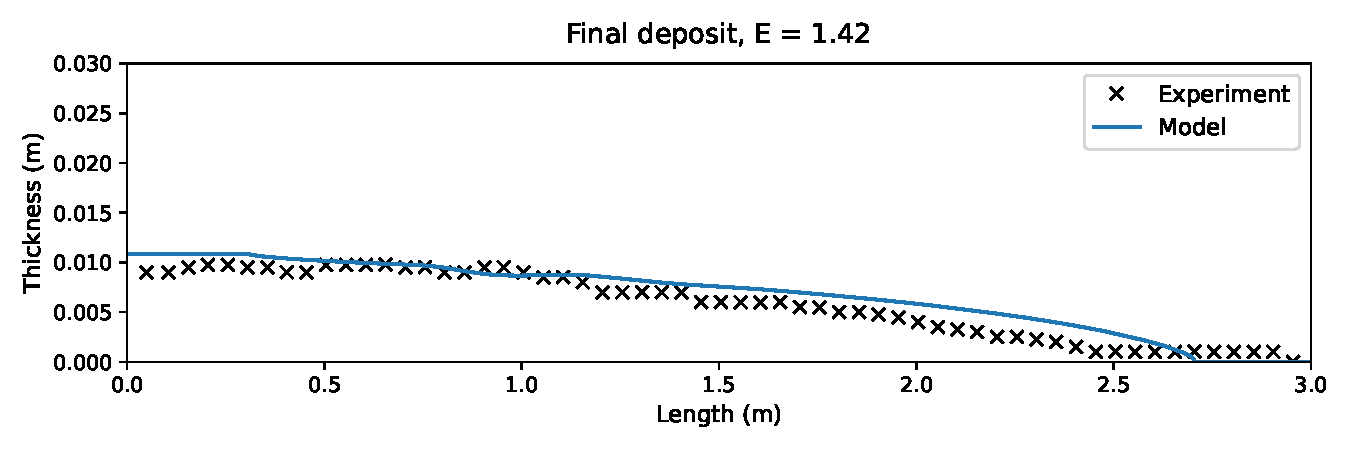
\includegraphics[width=0.45 \textwidth]{Figures/my_csed_E_1.42.pdf}\\
    \caption{Numerical and experimental results obtain in this study.}
    \label{fig:res}
\end{figure}
The original results are reproduced in figure~\ref{fig:Andrea}. In order to simplify the comparisons with the original article, in our plots, we also truncated the domain at $x=3$~m as nothing is happening in the right-hand side of the domain.
\begin{figure}[ht!]
    \centering
    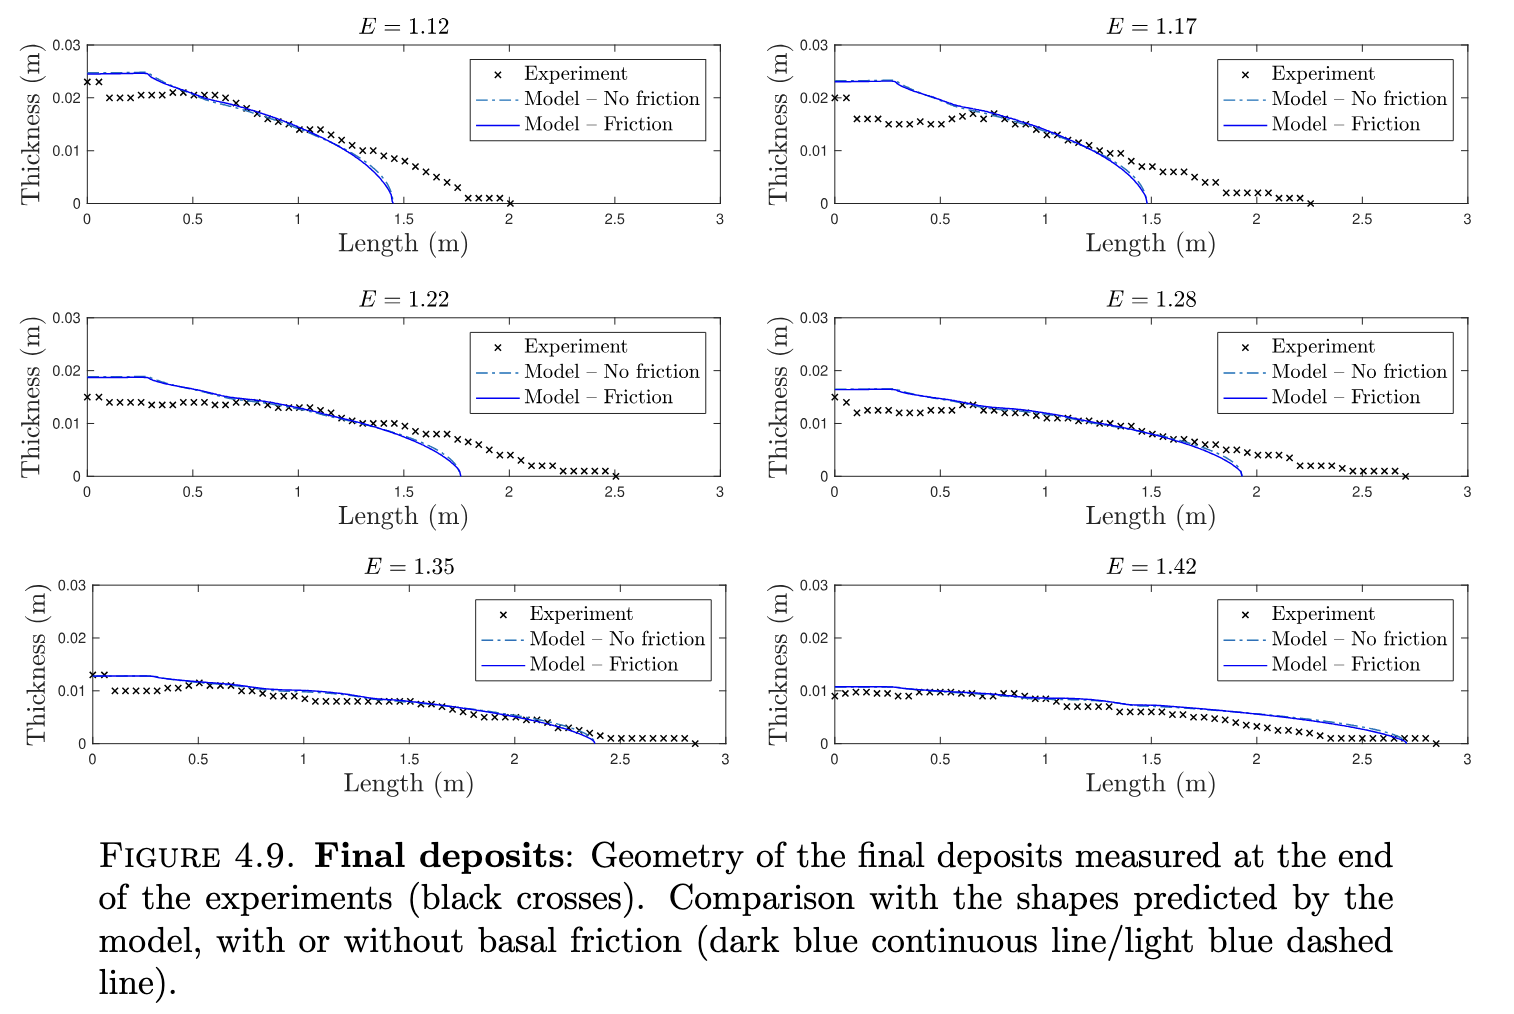
\includegraphics[width = 0.95 \textwidth]{Figures/ResAndrea.png}
    \caption{Numerical and experimental results obtained in the original work~\cite{Andrea}.}
    \label{fig:Andrea}
\end{figure}

As in the original article, one can note that, in figure~\ref{fig:res}, our experimental results are better fitted when the expansion is larger. If we now compare the two sets of numerical results with each other, the figures are very similar, regardless of the value of the expansion, between the original paper and this study.

\medskip

At this point, we were able to reproduce the results of the original article, based on the actual content of the article and on the bibliography. Starting with the same model, we implemented a numerical resolution following the steps of~\cite{Andrea}. However, as certain critical components were underspecified in the original work (the exact formulation choice of the HLL flux, the specifics of the optimization algorithm, and the choice of boundary conditions) specific implementation choices were necessary to perform the simulations.



\section{Comparison with the original results and prospects}\label{sec:comp}

At this point, we decided to ask the original authors to share their numerical results, in order to make a precise comparison of the deposit. Results are plotted in figure~\ref{fig:comp_opt} and figure~\ref{fig:comp}.

\begin{figure}[ht!]
    \centering
    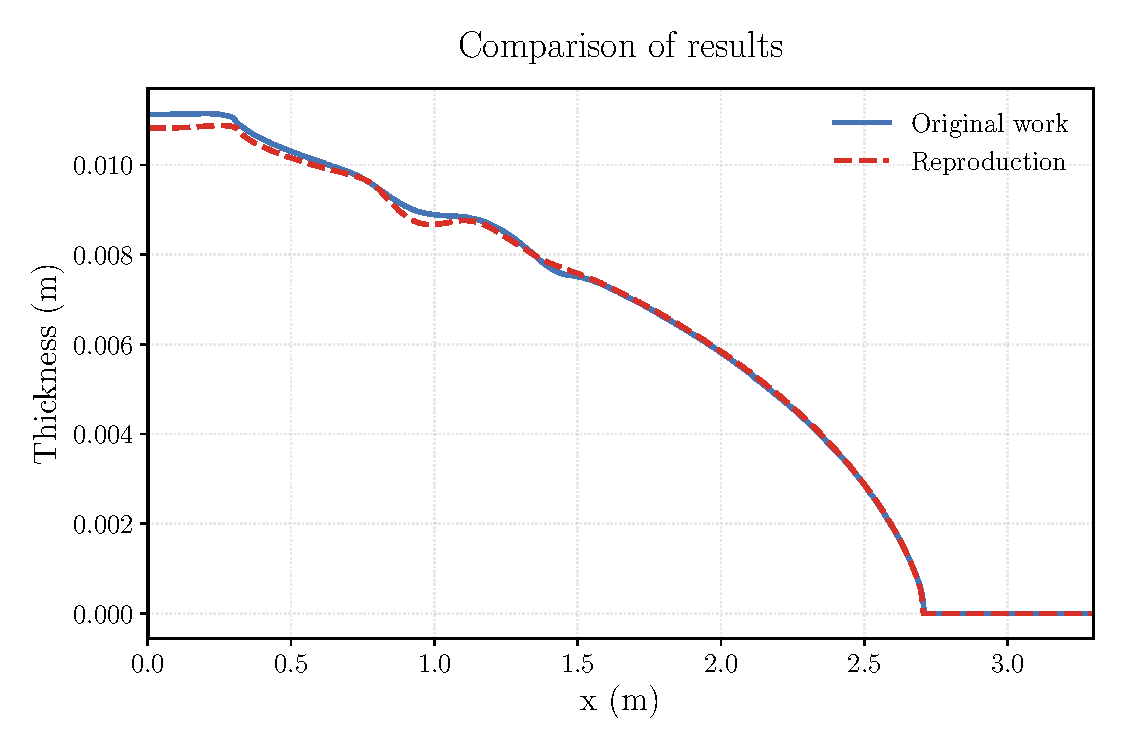
\includegraphics[width=0.9 \textwidth]{Figures/same_code_different_flux_hll_142_opt.pdf}
    \caption{Comparison of the numerical results for $E = 1.42$ with the $C_{sed}$ value found by the algorithm for each.}
    \label{fig:comp_opt}
\end{figure}
\begin{table}[!ht]
    \centering
    \caption{Comparison of $L^1$, $L^2$, and $L_{\infty}$ relative errors for various values of E with the $C_{sed}$ value found by the algorithm for each.}
    \begin{tabular}{llccc}
        \toprule
        \textbf{E} & \textbf{Code version} & $\mathbf{L^1}$ & $\mathbf{L^2}$ & $\mathbf{L_{\infty}}$ \\
        \midrule
        \multirow{2}{*}{1.12} & Original & 2.220045e-01 & 2.579376e-01 & 4.347826e-01 \\
                               & Reproduction  & 2.185487e-01 & 2.545067e-01 & 4.347826e-01 \\
        \midrule
        \multirow{2}{*}{1.17} & Original & 3.254562e-01 & 3.467081e-01 & 4.000000e-01 \\
                               & Reproduction  & 3.171704e-01 & 3.395263e-01 & 4.000000e-01 \\
        \midrule
        \multirow{2}{*}{1.22} & Original & 2.916570e-01 & 3.219815e-01 & 5.333333e-01 \\
                               & Reproduction  & 2.824498e-01 & 3.143024e-01 & 5.333333e-01 \\
        \midrule
        \multirow{2}{*}{1.28} & Original & 2.361637e-01 & 2.610457e-01 & 3.357710e-01 \\
                               & Reproduction  & 2.306824e-01 & 2.561719e-01 & 3.333333e-01 \\
        \midrule
        \multirow{2}{*}{1.35} & Original & 1.391942e-01 & 1.598507e-01 & 2.446122e-01 \\
                               & Reproduction  & 1.377796e-01 & 1.567616e-01 & 2.281177e-01 \\
        \midrule
        \multirow{2}{*}{1.42} & Original & 2.076277e-01 & 2.047887e-01 & 2.378280e-01 \\
                               & Reproduction  & 2.022209e-01 & 1.999374e-01 & 2.410582e-01 \\
        \bottomrule
    \end{tabular}
    \label{table:err-opt}
\end{table}

\begin{figure}[ht!]
    \centering
    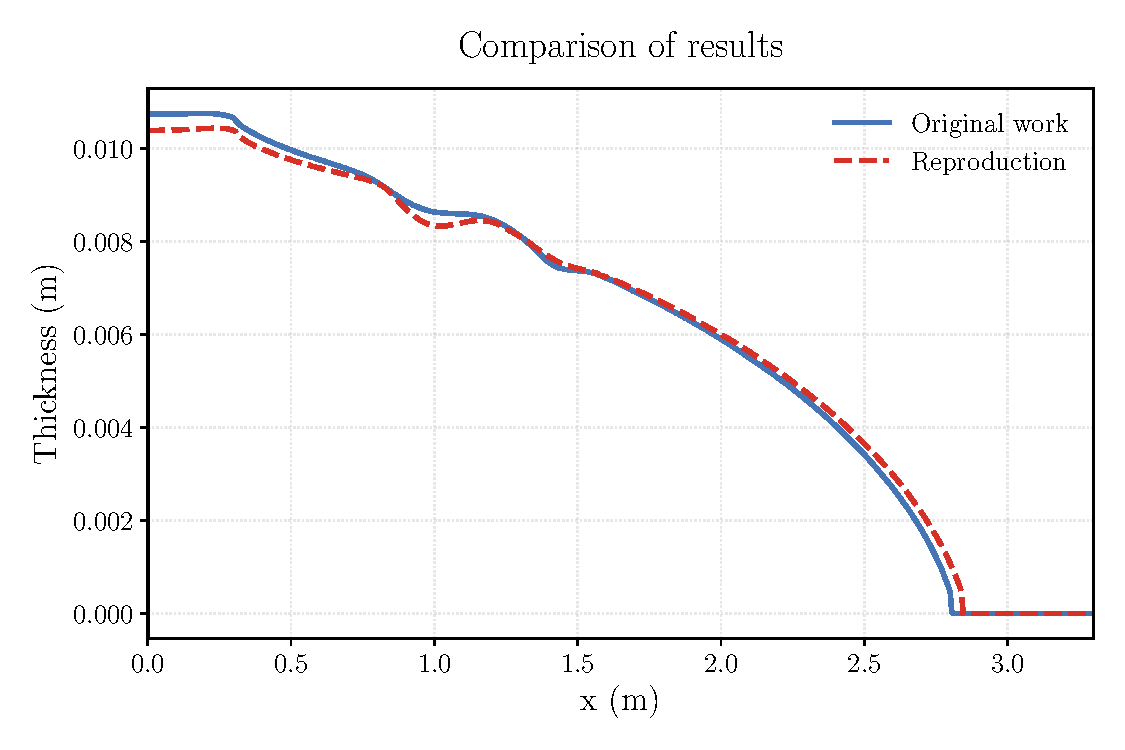
\includegraphics[width=0.9 \textwidth]{Figures/same_code_different_flux_hll1.pdf}
    \caption{Comparison of the numerical results for $E = 1.42$ with $C_{sed} = 3.113$.}
    \label{fig:comp}
\end{figure}

\begin{table}[!ht]
    \centering
    \caption{Comparison of $L^1$, $L^2$, and $L_{\infty}$ relative errors for various values of E with the $C_{sed}$ which were provided in equation~\eqref{eq:csed}.}
    \begin{tabular}{llccc}
        \toprule
        \textbf{E} & \textbf{Code version} & $\mathbf{L^1}$ & $\mathbf{L^2}$ & $\mathbf{L_{\infty}}$ \\
        \midrule
        \multirow{2}{*}{1.12} & Original & 2.247957e-01 & 2.606166e-01 & 4.347826e-01 \\
                               & Reproduction  & 2.185487e-01 & 2.545067e-01 & 4.347826e-01 \\
        \midrule
        \multirow{2}{*}{1.17} & Original & 3.300876e-01 & 3.506894e-01 & 4.038600e-01 \\
                               & Reproduction  & 3.171704e-01 & 3.395263e-01 & 4.000000e-01 \\
        \midrule
        \multirow{2}{*}{1.22} & Original & 2.996789e-01 & 3.319884e-01 & 5.333333e-01 \\
                               & Reproduction  & 2.824498e-01 & 3.143024e-01 & 5.333333e-01 \\
        \midrule
        \multirow{2}{*}{1.28} & Original & 2.463630e-01 & 2.713444e-01 & 3.633247e-01 \\
                               & Reproduction  & 2.306824e-01 & 2.561719e-01 & 3.333333e-01 \\
        \midrule
        \multirow{2}{*}{1.35} & Original & 1.527077e-01 & 1.725377e-01 & 2.573584e-01 \\
                               & Reproduction  & 1.377796e-01 & 1.567616e-01 & 2.281177e-01 \\
        \midrule
        \multirow{2}{*}{1.42} & Original & 2.076981e-01 & 2.041882e-01 & 2.334330e-01 \\
                               & Reproduction  & 2.022209e-01 & 1.999374e-01 & 2.410582e-01 \\
        \bottomrule
    \end{tabular}
    \label{table:err}
\end{table}

Figure~\ref{fig:comp_opt} presents a comparative analysis where each code is evaluated using its independently optimized $C_{sed}$ parameter. This approach highlights the difference between the two curves at the same endpoint.
Figure~\ref{fig:comp} enforces an identical $C_{sed}$. By freezing that parameter, this isolates and compares the pure implementation.

These figures, with $E=1.42$, are provided to illustrate the general behavior, which remains consistent across all six simulations, with the other values of $E$. While additional figures have been omitted to avoid redundancy, the specific relative errors for all six configurations are detailed in table~\ref{table:err-opt} and table~\ref{table:err}.

The two approximations are in agreement with the experiments. However, they slightly differ from one to the other. There is no evident reason to prefer a solution to the other.

After discussion with the authors of the original study, this difference comes from a different way to compute the eigenvalues.
The original version modifies the definition of the Riemann problem by introducing a coupling of eigenvalues between the two layers. Their code first calculates the wave speeds globally:
\begin{subequations}
\label{eq:c1c2orig}
\begin{align}
    c_1 &= \inf_{U = U_1^L, U_1^R, U_2^L, U_2^R} \left( \inf_{k = {1,2}} \lambda_k(U)\right)  = \inf_{U = U_1^L, U_1^R, U_2^L, U_2^R} \lambda_1(U) \label{eq:c1orig} \\
    c_2 &= \sup_{U = U_1^L, U_1^R, U_2^L, U_2^R} \left( \sup_{k = {1,2}} \lambda_k(U)\right) = \sup_{U = U_1^L, U_1^R, U_2^L, U_2^R} \lambda_2(U) \label{eq:c2orig}
\end{align}
\end{subequations}
and then calculates the flux using these global wave speeds
\begin{align*}
    f_{\Delta x}(U_j^L,U_j^R) = \begin{cases}
        F(U_j^L) &\text{if $0 < c_1$}\\
        \dfrac{c_1 F(U_j^L) - c_2 F(U_j^R)}{c_2 - c_1}+ \dfrac{c_1 c_2}{c_2-c_1}(U_j^R-U_j^L) &\text{if $c_1 < 0 < c_2$}\\
        F(U_j^R) &\text{if $c_2 < 0$}.
    \end{cases}
\end{align*}
One can refer to figure~\ref{fig:velocities} to illustrate the differences between the solutions of equations~\eqref{eq:c1c2repro} and the solutions of equations~\eqref{eq:c1c2orig}.
% \begin{figure}[htbp]
%     \centering

%     \begin{tikzpicture}[>=stealth, thick, scale=0.8]

%         \draw[->] (-6,0) -- (6.5,0) node[right] {$\lambda$};
%         \draw[->] (0,-0.5) -- (0,4.5) node[above] {$t$};
%         \node[below left] at (0,0) {$0$};

%         \foreach \x/\col/\lab in {
%             -4.5/red/{c_1 = c_1^{(1)}\qquad}, -3.5/blue/{c_1^{(2)}}, -1.5/blue/{},
%             1.0/red/{}, 2.0/red/{}, 3.0/red/{\quad c_2^{(1)}}, 4.5/blue/{}, 5.5/blue/{\qquad \qquad c_2 = c_2^{(2)}}
%         } {
%             \draw[\col, ->] (0,0) -- (\x, 3.5)
%                 node[anchor=south, inner sep=2pt, font=\small, text=\col] {$\lab$};
%         }
%     \end{tikzpicture}

%     \caption{Representation of wave velocities: example where the first layer velocities $c_1^{(1)}$ and $c_1^{(2)}$ are given by equation~\eqref{eq:c1repro}, the second layer velocities $c_2^{(1)}$ and $c_2^{(2)}$ are given by  equation~\eqref{eq:c2repro} while $c_1$ and $c_2$ are globally computed by~\eqref{eq:c1orig} and by~\eqref{eq:c2orig} respectively. }
%     \label{fig:velocities}
% \end{figure}
\begin{figure}[htbp]
    \centering

    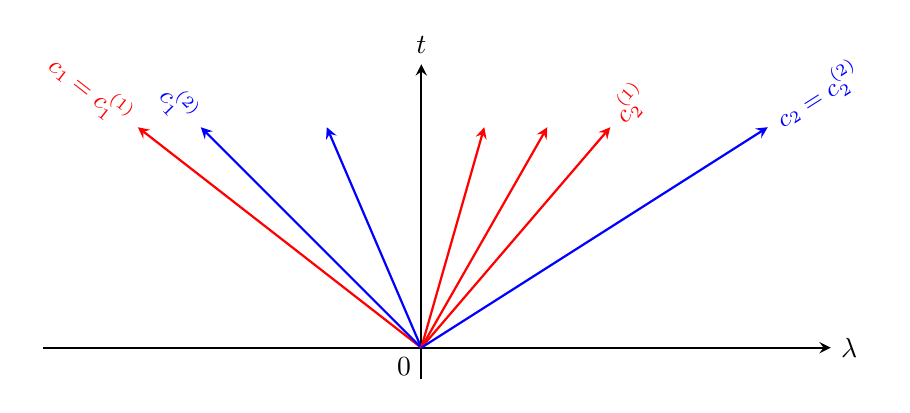
\begin{tikzpicture}[>=stealth, thick, scale=0.8]
        \draw[->] (-6,0) -- (6.5,0) node[right] {$\lambda$};
        \draw[->] (0,-0.5) -- (0,4.5) node[above] {$t$};
        \node[below left] at (0,0) {$0$};

        \coordinate (c1_1_tip) at (-4.5, 3.5);
        \coordinate (c1_2_tip) at (-3.5, 3.5);
        \draw[red, ->] (0,0) -- (c1_1_tip);
        \draw[blue, ->] (0,0) -- (c1_2_tip);
        \draw[blue, ->] (0,0) -- (-1.5, 3.5);

        \draw[red, ->] (0,0) -- (1.0, 3.5);
        \draw[red, ->] (0,0) -- (2.0, 3.5);
        \coordinate (c2_1_tip) at (3.0, 3.5);
        \coordinate (c2_2_tip) at (5.5, 3.5);
        \draw[red, ->] (0,0) -- (c2_1_tip);
        \draw[blue, ->] (0,0) -- (c2_2_tip);

        \node[anchor=east, rotate={atan2(3.5,-4.5)+180}, red, inner sep=4pt, font=\small]
            at (c1_1_tip) {$c_1 = c_1^{(1)}$};

        \node[anchor=east, rotate={atan2(3.5,-3.5)+180}, blue, inner sep=4pt, font=\small]
            at (c1_2_tip) {$c_1^{(2)}$};

        \node[anchor=west, rotate={atan2(3.5,3.0)}, red, inner sep=4pt, font=\small]
            at (c2_1_tip) {$c_2^{(1)}$};

        \node[anchor=west, rotate={atan2(3.5,5.5)}, blue, inner sep=4pt, font=\small]
            at (c2_2_tip) {$c_2 = c_2^{(2)}$};

    \end{tikzpicture}

    \caption{Representation of wave velocities: example where the minimum velocities for each layer $c_1^{(1)}$ and $c_1^{(2)}$ are given by equation~\eqref{eq:c1repro}, the maximum velocities $c_2^{(1)}$ and $c_2^{(2)}$ are given by  equation~\eqref{eq:c2repro} while $c_1$ and $c_2$ are globally computed by~\eqref{eq:c1orig} and by~\eqref{eq:c2orig} respectively.}
    \label{fig:velocities}

\end{figure}

This difference in the computation of the wave speeds therefore inevitably implies values of $C_{sed}$ that differ from those found in Section 4.

A more in-depth analysis must be carried out to analyse these differences. A comparison with analytical solutions should also be a way to pursue this study.


\section*{Acknowledgments}
This work was founded by the France 2030 program "ANR-23-EXMA-0004" (PEPR Maths-Vives) through the Complexflows project.
